\section{Resultados}

\subsection{Ejecución}

\begin{enumerate}
	\item Defecto en la cadena
	      	          
	\item Normalización
	      	          
\end{enumerate}

\begin{figure}
	\centering
	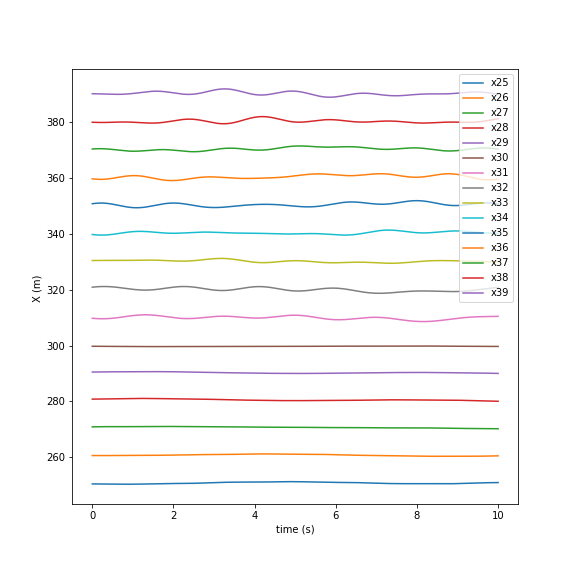
\includegraphics[width=0.4\textwidth]{seq_n30.png}
	\caption{Plot x25 a x40 en tiempo para n0 = 30}
\end{figure}

\begin{figure}
	\centering
	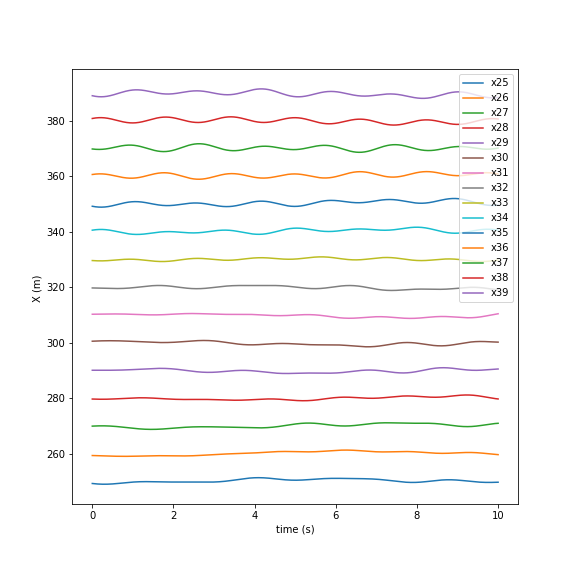
\includegraphics[width=0.4\textwidth]{seq_n60_30.png}
	\caption{Plot x25 a x40 en tiempo para n0 = 60}
\end{figure}

\begin{figure}
	\centering
	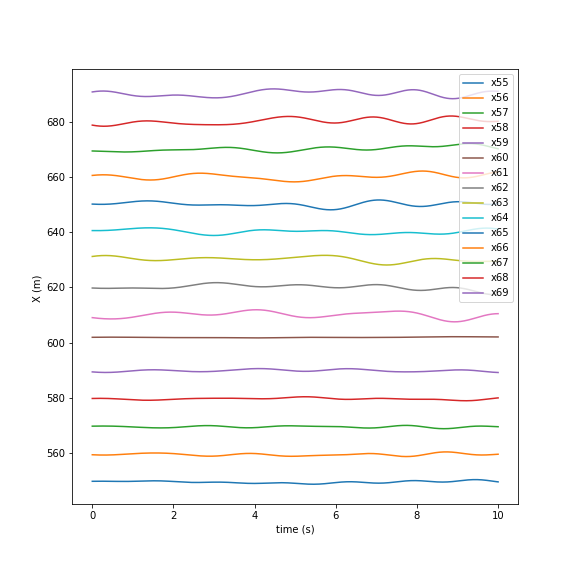
\includegraphics[width=0.4\textwidth]{seq_n60_60.png}
	\caption{Plot x55 a x70 en tiempo para n0 = 60}
\end{figure}



Elevar la dimensión de la cadena. Obtener mediciones significativas de tiempos.

\subsection{Simulaciones}
% b) Registrar el desarrollo de las simulaciones de manera ordenada en por lo menos 3 pasos (versiones beta)
Primer paso
Segundo paso
Tercer paso

\subsection{Complejidad}

Teorico:

\begin{itemize}
	\item \textbf{Secuencial}:
	      hola
	\item \textbf{Paralelo}:
	      	          
\end{itemize}

Comparación con experimental, tiempo. Incluir graficos

\subsection{Velocidad}

Medir velocidad del algoritmo en FLOPs. graficos

Medir la escalabilidad del software

e) Optimizar el software con un desarrollo orientado al paralelismo, y presentarlo
en las conclusiones del paper